% Domain and boundary conditions of the cover run (04.11.2026). Build: pdflatex domain.tex, then
% magick -density 300 domain.pdf -background white -alpha remove domain.png
\documentclass[tikz,border=6pt]{standalone}
\usepackage{amsmath}
\usetikzlibrary{arrows.meta,decorations.pathmorphing,patterns}
\begin{document}
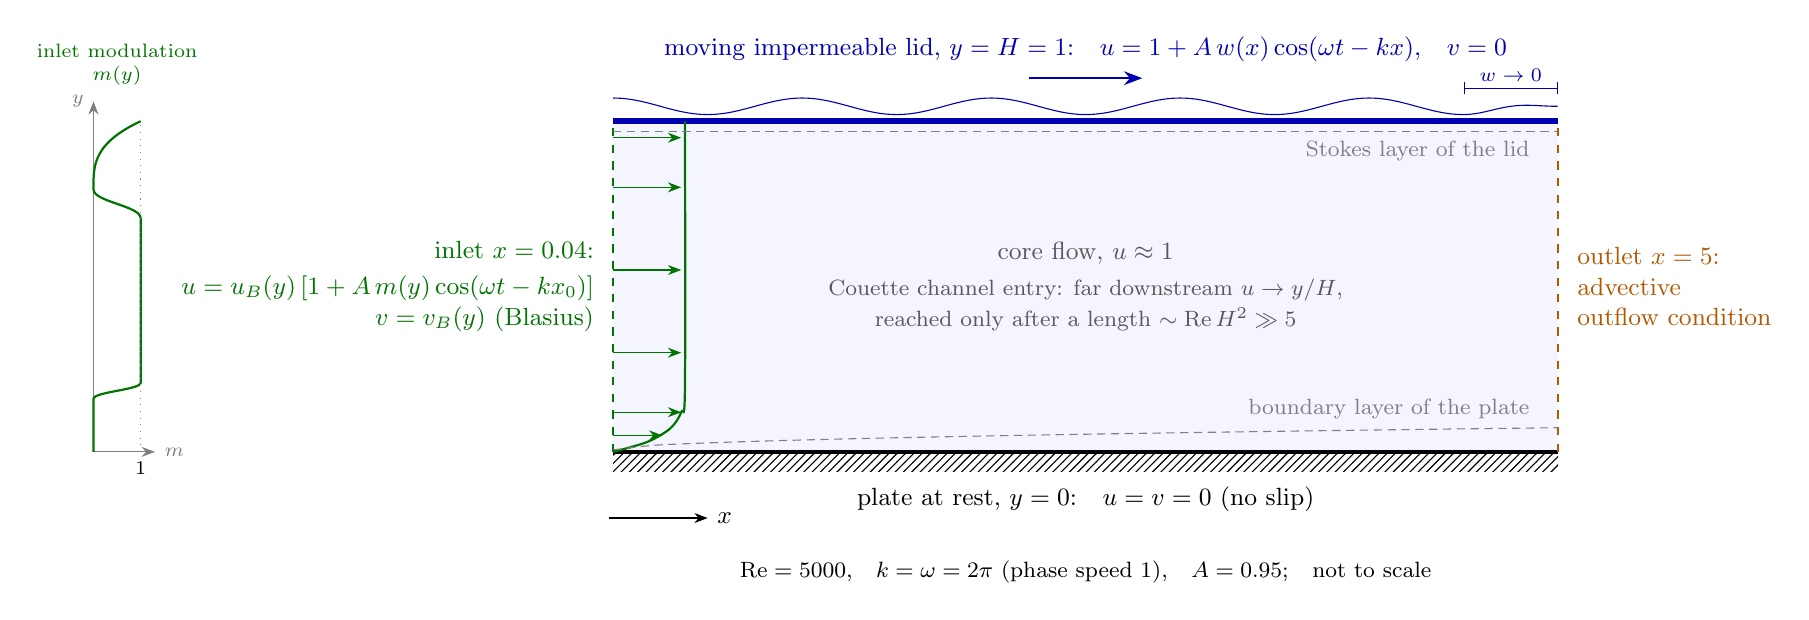
\begin{tikzpicture}[x=2.4cm,y=4.2cm,>=Stealth,font=\small]
  \def\L{5}\def\H{1}
  \colorlet{lid}{blue!70!black}\colorlet{inl}{green!45!black}\colorlet{outl}{orange!70!black}
  % domain
  \fill[blue!4] (0,0) rectangle (\L,\H);
  % plate with hatching
  \fill[pattern=north east lines] (0,-0.06) rectangle (\L,0);
  \draw[very thick] (0,0) -- (\L,0);
  \node[below=9pt] at (\L/2,0) {plate at rest, $y=0$:\quad $u=v=0$ (no slip)};
  % lid
  \draw[line width=2pt,lid] (0,\H) -- (\L,\H);
  \draw[lid,domain=0:\L,samples=200,smooth] plot (\x,{\H+0.045+0.025*cos(deg(2*pi*\x))*(\x<4.5 ? 1 : 0.5*(1+cos(deg(pi*(\x-4.5)/0.5))))});
  \draw[->,lid,thick] (2.2,\H+0.13) -- (2.8,\H+0.13);
  \node[lid,above] at (\L/2,\H+0.15) {moving impermeable lid, $y=H=1$:\quad
    $u=1+A\,w(x)\cos(\omega t-kx)$,\quad $v=0$};
  \draw[lid,|-|] (4.5,\H+0.10) -- (5,\H+0.10) node[midway,above=-1pt,font=\scriptsize] {$w\to0$};
  % inlet
  \draw[inl,thick,dashed] (0,0) -- (0,\H);
  \draw[inl,thick] plot[smooth] coordinates {(0,0) (0.18,0.03) (0.30,0.07) (0.36,0.12) (0.38,0.2) (0.38,\H)};
  \foreach \yy in {0.05,0.12,0.3,0.55,0.8,0.95} {
    \pgfmathsetmacro{\ux}{\yy<0.12 ? 0.20+1.2*\yy : 0.36}
    \draw[->,inl] (0,\yy) -- (\ux,\yy);}
  \node[inl,align=right,left] at (-0.05,\H/2) {inlet $x=0.04$:\\[2pt]
    $u=u_B(y)\,[1+A\,m(y)\cos(\omega t-kx_0)]$\\ $v=v_B(y)$ (Blasius)};
  % modulation m(y) sketch
  \begin{scope}[shift={(-2.75,0)},x=0.6cm]
    \draw[->,gray] (0,0) -- (0,\H+0.06) node[left,font=\scriptsize] {$y$};
    \draw[->,gray] (0,0) -- (1.3,0) node[right,font=\scriptsize] {$m$};
    \draw[inl,thick] (0,0) -- (0,0.157) plot[domain=0:1,samples=30] ({\x-sin(deg(2*pi*\x))/(2*pi)},{0.157+0.0555*\x}) -- (1,0.70)
      plot[domain=0:1,samples=30] ({1-(\x-sin(deg(2*pi*\x))/(2*pi))},{0.70+0.1*\x}) plot[domain=0:1,samples=30] ({\x^3},{0.8+0.2*\x});
    \node[inl,font=\scriptsize,align=center,above] at (0.5,\H+0.08) {inlet modulation\\ $m(y)$};
    \draw[gray,dotted] (1,0) -- (1,\H);
    \node[below,font=\scriptsize] at (1,0) {1};
  \end{scope}
  % outlet
  \draw[outl,thick,dashed] (\L,0) -- (\L,\H);
  \node[outl,align=left,right] at (\L+0.05,\H/2) {outlet $x=5$:\\ advective\\ outflow condition};
  % layers inside
  \draw[gray,densely dashed] plot[smooth,domain=0:\L] (\x,{0.006+0.03*sqrt(\x)});
  \node[gray,font=\footnotesize,above left] at (\L-0.1,0.07) {boundary layer of the plate};
  \draw[gray,densely dashed] (0,\H-0.03) -- (\L,\H-0.03);
  \node[gray,font=\footnotesize,below left] at (\L-0.1,\H-0.03) {Stokes layer of the lid};
  \node[gray!70!black,align=center] at (\L/2,\H/2) {core flow, $u\approx 1$\\[2pt]
    \footnotesize Couette channel entry: far downstream $u\to y/H$, \\ \footnotesize reached only after a length $\sim \mathrm{Re}\,H^2 \gg 5$};
  % axes
  \draw[->] (-0.02,-0.2) -- (0.5,-0.2) node[right] {$x$};
  \node[below,font=\footnotesize] at (\L/2,-0.30) {$\mathrm{Re}=5000$,\quad $k=\omega=2\pi$ (phase speed $1$),\quad $A=0.95$;\quad not to scale};
\end{tikzpicture}
\end{document}
